This section describes the possible events that may happen in the
problem domain. These events and the classes affected by them, will be
described through an event table and a state diagram for each class
described in \cref{sub:pd_classes}.

\begin{description}

\item[Submitting/Cancelling votes]
    When a user votes for a track, or cancels it. If the \emph{Track} that is voted for fits within the \emph{Restriction}, the \emph{Track}s vote count is changed and potentially its order in the \emph{Playlist}. The specific \emph{User}s vote is also changed.

\item[Checking in/out of venues]
    A \emph{User} checks in at a venue. This allows the user to vote
    for \emph{Tracks} on the venue's playlist.

\item[Searching for a track]
    When a \emph{User} is searching for a desired \emph{Track} in the catalogue of \emph{Track}s. The \emph{User} should receive relevant search results that fit within the \emph{Restriction}s.

\item[Adding/Removing a track from the \emph{Playlist}]
    Tracks can be added to the playlist by a \emph{User} voting on a
    \emph{Track}. A \emph{Track} can be removed from the playlist if
    either its votes were cancelled, or if the \emph{Track} was just played.

\item[New track is playing]
    This event happens when a \emph{Track} has ended, due to it being skipped or
    reaching the end. This should affect the vote count of the
    \emph{Track}. If the \emph{Track} a \emph{User} has voted
    for is played, the \emph{User}s vote should be reset, and the
    \emph{Track} that ended should be added to the history.

\item[Adding/Removing restrictions]
    When the administrator either adds or removes a \emph{Restriction} from the \emph{Playlist}. \emph{Track}s on the \emph{Playlist} that do not meet the \emph{Restriction}s should be removed. The \emph{User}s' votes should also be voided if it does not meet the \emph{Restriction}.

\end{description}

The following event table is used to describe what classes are involved in the immediate events of the problem domain.

\begin{table}[htbp]
    \centering
    \tabcolsep=0.10cm
    \begin{tabular}{lccccccc}
        \toprule
        \textbf{Events}                 & User   & Track  & Playlist & Vote   & Restriction & Venue  & History\\
        \midrule
        (Re)vote                        & $\ast$ & $\ast$ &   $\ast$ &   $+$  &             &        &        \\
        User checks in at venue         & $+$    &        &          &        &             & $+$    &        \\
        User leaves venue               & $+$    &        &          &  $+$   &             & $+$    &        \\
        User searches for a track       & $\ast$ &  $+$   &          &        & $\ast$      &        &        \\
        Track added to playlist         & $\ast$ & $\ast$ & $\ast$   & $+$    &             &        &        \\
        Track removed from playlist     &        & $+$    & $\ast$   & $+$    &             &        &        \\
        A new track is playing          &        & $\ast$ & $\ast$   & $+$    &             &        & $\ast$ \\
        Restriction activated           &        &        & $\ast$   &        & $\ast$      &        &        \\
        Restriction deactivated         &        &        & $\ast$   &        & $\ast$      &        &        \\
        \bottomrule
    \end{tabular}
    \caption{Event table for the problem domain.}\label{eventtable}
\end{table}

In \cref{eventtable}, the different events in the problem domain and
what objects are effected by these are mapped. Stars ($\ast$) mean that the
event can occur zero or more times. Pluses ($+$) mean that the event can
occur zero or one times. From this, specific state diagrams can be created to illustrate how the objects are created, affected and terminated.

\begin{figure}[H]
  \centering
  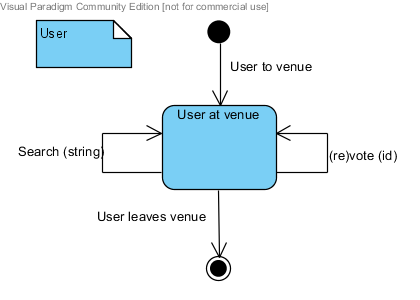
\includegraphics[width=.7\textwidth]{StateDiagramUser.png}
  \caption{State diagram for the user.}\label{fig:StateDiagramUser}
\end{figure}

In \cref{fig:StateDiagramUser} the state diagram for a user can be seen. The problem domain is the context of the venue, and a user can therefore only affect the problem domain, when he or she is present at the venue. This results in the creation of the user, when he or she enters, and the termination when he or she leaves. When present at the venue, the user can search for tracks and vote or revote for these.

\begin{figure}[H]
  \centering
  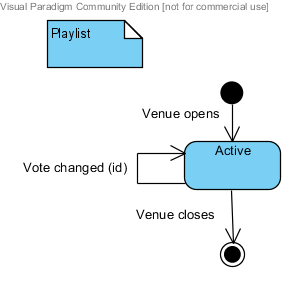
\includegraphics[width=.7\textwidth]{StateDiagramPlaylist.png}
  \caption{State diagram for the playlist.}\label{fig:StateDiagramPlaylist}
\end{figure}

In \cref{fig:StateDiagramPlaylist} it can be seen that a playlist, is created when the venue opens, and terminated when it closes. The playlist automatically plays the next track, and users can change their votes as desired.

\begin{figure}[H]
  \centering
  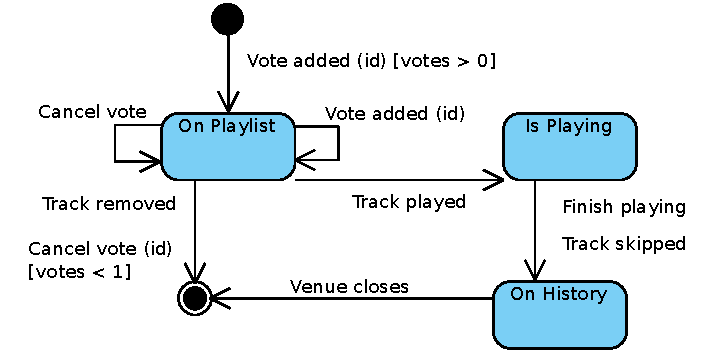
\includegraphics[width=.7\textwidth]{StateDiagramTrack.pdf}
  \caption{State diagram for the track.}\label{fig:StateDiagramTrack}
\end{figure}

As seen in \cref{fig:StateDiagramTrack}, a track is only active in
the problem domain, when it has votes or is on the history of last
played tracks. This means that it will be created, when it receives
its first vote. If votes are removed from the track, it can result in
the track having zero votes again, and will therefore be
terminated. While active, the track can receive and lose votes from
any user when the user's vote is changed. A track is terminated once it has
been removed from the history of last played tracks.

\begin{figure}[H]
  \centering
  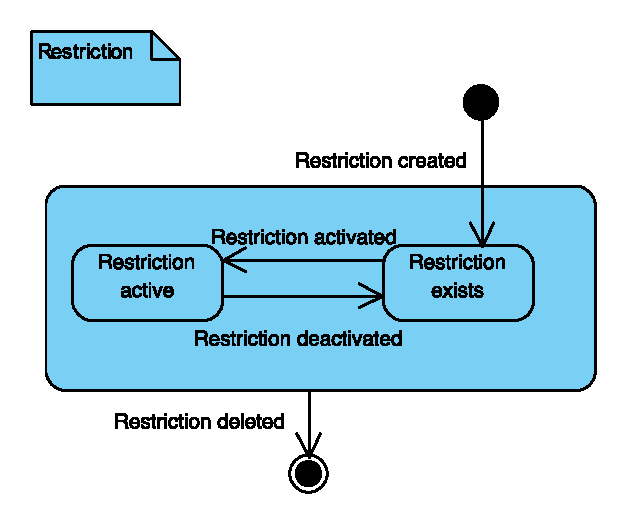
\includegraphics[width=.7\textwidth]{StateDiagramRestriction.pdf}
  \caption{State diagram for the restriction.}\label{fig:StateDiagramRestriction}
\end{figure}

As shown in \cref{fig:StateDiagramRestriction}, a restriction can be created and deleted at any time. This can only be done by the administrator. A restriction only affect the users' searches when it is active. It can be toggled between active and inactive by the administrator or the system at any time.

\begin{figure}[H]
  \centering
  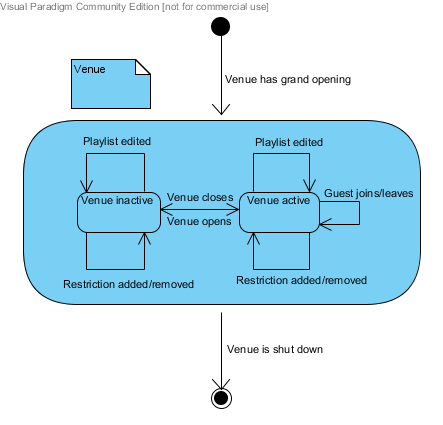
\includegraphics[width=.7\textwidth]{pd_venueState.png}
  \caption{State diagram for the venue.}\label{fig:StateDiagramVenue}
\end{figure}

As shown in \cref{fig:StateDiagramVenue}, a venue is created when it first opens and is terminated when it is shut down. A venue has only two states, active and inactive, meaning whether or not guests are allowed. A venue can edit its playlist, without changing state, and likewise add or remove restrictions.

\begin{figure}[H]
  \centering
  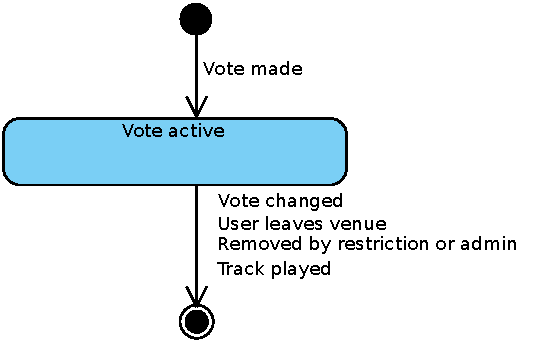
\includegraphics[width=.7\textwidth]{StateDiagramVote.pdf}
  \caption{State diagram for vote class.}\label{fig:StateDiagramVote}
\end{figure}

\Cref{fig:StateDiagramVote} describes the vote class. This class is very simple. It is created when a user votes on a track, and is terminated when the user, that created the vote, changes his/her vote, thereby cancelling the old vote. It also terminates when the track the vote on is is played, the administrator removes the vote or the user leaves, thereby cancelling all his or her votes.

\begin{figure}[H]
  \centering
  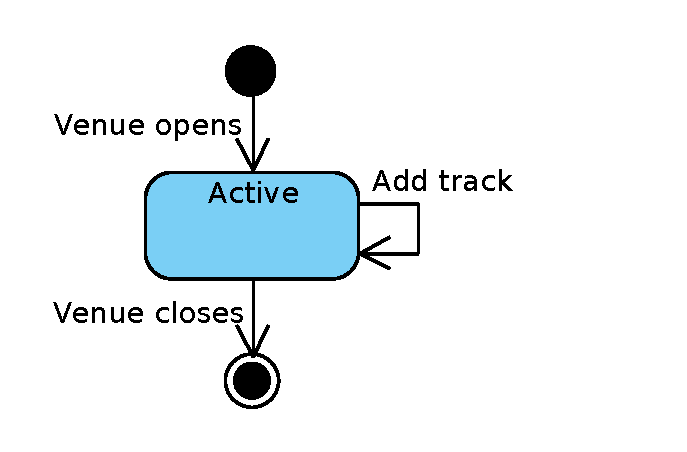
\includegraphics[width=.7\textwidth]{StateDiagramHistory.pdf}
  \caption{State diagram for history class.}\label{fig:StateDiagramHistory}
\end{figure}

\Cref{fig:StateDiagramHistory} describes the history class. When the venue opens, the history is active. When a new track is playing, the previously playing track is added to the history.
